\section{Введение}

\textbf{Цель работы:}
определение коэффициента теплопроводности воздуха или углекислого газа при атмосферном давлении и разных температурах по теплоотдаче нагреваемой током нити в цилиндрическом сосуде.

\textbf{В работе используются:}
прибор для определения теплопроводности газов; форвакуумный насос; газгольдер с углекислым газом; манометр; магазин сопротивлений; эталонное сопротивление 10 Ом; цифровой вольтметр В7-38; источник питания.

\subsection{Теоритические сведения}

Основные сведения о теплопроводности газов содержатся в описании к предыдущей работе. Разрешая $T_1 - T_2 = \frac{Q}{2\pi L\varkappa} \ln\frac{r_2}{r_1}$ относительно $\varkappa$, получим
\begin{equation}
    \varkappa = \frac{Q}{2\pi L \left(T_1 - T_2\right)} \ln \frac{r_2}{r_1}
\end{equation}
где $r_1$ — радиус нити, $r_2$ — радиус внешнего цилиндра, $Q$ -- тепловой поток, $T_1$ -- темперкатура нити, $T_2$ -- температура цилиндра, $\varkappa$ -- коэффициент теплопроводности воздуха, $L$ -- длина цилиндра и нити.

Предлагаемый в работе метод измерения теплопроводности газов основан на применении формулы (1).

\subsection{Эксперементальная установка}

Схема установки изображена на рисунке 1. Тонкая нить (никелевая или вольфрамовая проволока) натянута по оси длинной вертикально стоящей медной трубки. Через
штуцер трубка заполняется исследуемым газом. Нить нагревается электрическим током, ее температура $T_1$ определяется по изменению электрического сопротивления. Трубка находится в кожухе, через который пропускается вода из термостата. Температура воды $T_2$ измеряется термометром, помещенным в термостат. Количество теплоты, протекающей через газ, равно (если пренебречь утечками тепла через торцы) количеству теплоты, выделяемому током в нити, и может быть найдено по закону Джоуля—Ленца. При этом ток в нити
определяется по напряжению на включенном последовательно с ней
эталонном сопротивлении 10 Ом. Таким образом, все величины, входящие в правую часть формулы (1), поддаются непосредственному
измерению.

\begin{figure}[h]
    \centering
    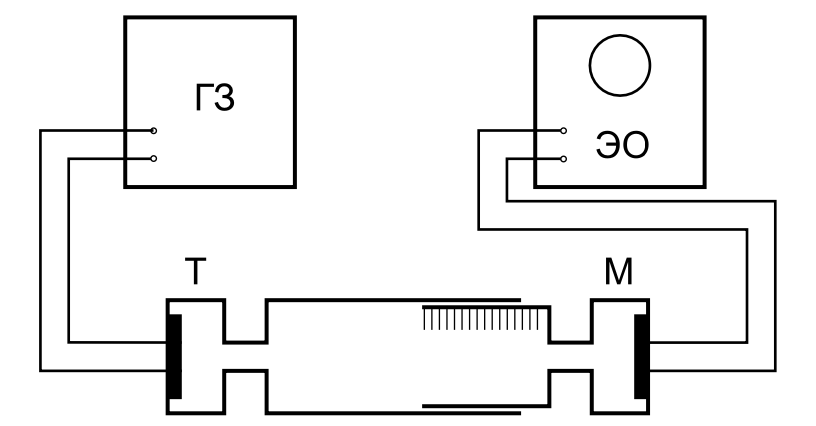
\includegraphics[width = 0.7\linewidth]{p1.png}
    \caption{Схема установки для определения теплопроводности газов}
\end{figure}

Электрическая часть схемы состоит из источника питания и подключенных к нему последовательно соединенных нити, эталонного сопротивления 10 Ом и магазина сопротивлений $R_\text{м}$, служащего для точной установки тока через нить. Цифровой вольтметр может подключаться как к нити, так и к эталонному сопротивлению, измеряя таким образом напряжение на нити и ток через нее.

Опыты проводят с воздухом или с углекислым газом (по указанию преподавателя) при атмосферном давлении. Предварительно — для удаления примесей — трубку несколько раз откачивают форвакуумным насосом и промывают исследуемым газом.

При определенной температуре термостата снимается зависимость напряжения на нити от тока, проходящего через нее. Затем по полученным данным строится график зависимости рассеиваемой мощности от сопротивления нити, по которому можно определить сопротивление нити при нулевом токе, то есть при температуре термостата. Это сопротивление затруднительно измерить непосредственно из-за термоэлектрических явлений, заметно искажающих результаты при малых токах, большие же токи существенно изменяют температуру нити. Повторив эти измерения при различных температурах термостата, можно определить температурную зависимость сопротивления нити. Коэффициент теплопроводности определяется затем по
зависимости выделяемой мощности от разности температур с помощью формулы (1). При небольших значениях разности температур эта зависимость хорошо аппроксимируется прямой.

При измерении теплопроводности газов необходимо иметь в виду, что целый ряд факторов может повлиять на результат опыта. Мы уже говорили о конвективном переносе тепла. Часть тепловой энергии передается от нити к стенке через излучение. Формула (1) не учитывает также потерь тепла через концы проволоки. Как показывают расчеты, при наших условиях опыта они вносят наиболее существенную погрешность (порядка нескольких процентов).
